\providecommand{\main}{../..}%define path to bib for subfiles
\documentclass[../../main.tex]{subfiles}
\begin{document}
\onlyinsubfile{\setcounter{chapter}{8}}
\notinsubfile{}
\chapter{microsoft videocast}


\hrefqr[-1cm]{https://www.youtube.com/watch?v=F_Riqjdh2oM}{youtube}
Op de \hrefqr[1cm]{https://www.microsoft.com/en-us/research/video/quantum-computing-computer-scientists/}{microsoft site} dezelfde film, maar met extra info.

Computers werken met bits, dat zijn twee-toestand modellen, waar of onwaar, nul of \'e\'en, kop of munt. In een computer wordt met spanningen gerekend. Transistoren zijn de schakelaars die door een programma aan of uitgezet worden. We kunnen daar ingewikkelde dingen mee doen, maar daar houdt de vergelijking met een quantum computer zo'n beetje op.

\begin{center}  %DE manier om figuur te ontfloaten.
\leavevmode
\begin{tikzpicture}[scale=.5]
\def\vectsize{.7}
\def\radius{5cm}
\def\labelrad{4.cm}
\def\ketrad{5.9cm}
\def\arrowrad{3cm}

\draw[color=black] (+90:\radius) -- (+270:0.1\radius);
\draw[color=black] (+0:\radius) -- (+180:0.1\radius);
\draw[color=black] (+0:\radius) -- (+90:\radius);
\filldraw (\radius/2, \radius/2) circle (.1);
\end{tikzpicture}
\captionof{figure}{Een klassiekbit, muntje opgooien \label{fig:coinflip}}
\end{center}

Als we een muntje opgooien geldt kans op munt + kans op kop =1.
Een eerlijk muntje zal met gelijke kans kop of munt geven.

We kunnen die toestand weergeven als een vector 
$\begin{pmatrix}
\tfrac{1}{2}\\
\tfrac{1}{2}
\end{pmatrix}$
of 
$\begin{pmatrix}
\tfrac{1}{6}\\
\tfrac{5}{6}
\end{pmatrix}$
als we bijvoorbeeld de uitkomst=drie of geen drie als basis nemen.

Er is een groot verschil met quantum computers. Hiervoor meoten we even wat lineaire alebra ophalen.

\subsection{lineaire algebra}
We gebruiken de eenheidsvectoren $\begin{pmatrix}
1\\
0
\end{pmatrix}$
 en $\begin{pmatrix}
1\\
1
\end{pmatrix}$
om de twee toestanden van een bit te defini\"eren.

Bit met waarde $0 \equiv \begin{pmatrix}
1\\
0
\end{pmatrix}
\equiv
\ket{0}$

Bit met waarde $1 \equiv 
\begin{pmatrix}
0\\
1
\end{pmatrix}
\equiv
\ket{1}$

\marginpar{\vspace{-3cm}
Definitie:\\
$0 \equiv \begin{pmatrix}
1\\
0
\end{pmatrix}
\equiv
\ket{0}$
}
\marginpar{\vspace{0cm}

Definitie:\\
$1 \equiv \begin{pmatrix}
0\\
1
\end{pmatrix}
\equiv
\ket{1}$}

(braket notatie nog niet ingevoerd.)

(matrix)(kolomvector=(kolomvector):

$
\begin{pmatrix}
a&b\\
c&d
\end{pmatrix}
\begin{pmatrix}
x\\
y
\end{pmatrix}
=
\begin{pmatrix}
ax+by\\
cx+dy
\end{pmatrix}
$

\easy Bereken de uitkomst van de volgende vectoroperatie

$
\begin{pmatrix}
1&0&0&0&0\\
0&0&1&0&0\\
0&1&0&0&0\\
0&0&0&0&1
\end{pmatrix}
\begin{pmatrix}
0\\
1\\
0\\
1
\end{pmatrix}
=
\begin{pmatrix}
0\\
0\\
1\\
1
\end{pmatrix}
$

\subsubsection{matrixvermenigvuldiging}
(matrix)(matrix)=(matrix)
Een product van twee matrices levert een nieuwe matrix op. Je vindt de elementen van de nieuwe matrix door de elementen van rijen van de linker matrix paarsgewijs te vermenigvuldigen met elementen van kolommen uit de rechter matrix. Je vindt dan het element op het kruispunt van de rij en kolom. De matrix moet vierkant zijn, anders werkt het niet.


$
\begin{pmatrix}
a&b\\
c&d
\end{pmatrix}
\begin{pmatrix}
p&q\\
r&s
\end{pmatrix}
=
\begin{pmatrix}
ap+br&aq+bs\\
cp+dr&cq+ds
\end{pmatrix}
$

We geven een voorbeeld in twee dimensies. 
Als we op een toestand $\begin{pmatrix}
a\\
b
\end{pmatrix}$
eerst de X-operator loslaten en vervolgens de Z operator, dan ziet dat er alsvolgt uit.
$
\begin{pmatrix}
1&0\\
0&-1
\end{pmatrix}
\begin{pmatrix}
0&1\\
1&0
\end{pmatrix}
\begin{pmatrix}
a\\
b
\end{pmatrix}
=
\begin{pmatrix}
1&0\\
0&-1
\end{pmatrix}
\begin{pmatrix}
b\\
a
\end{pmatrix}
=
\begin{pmatrix}
b\\
-a
\end{pmatrix}
$

\marginpar{$X=
\begin{pmatrix}
0&1\\
1&0
\end{pmatrix}
$}
\marginpar{$Z=
\begin{pmatrix}
1&0\\
0&-1
\end{pmatrix}
$}
Hetzelfde resultaat bereik je als je eerst de matrixen vermenigvuldigt: 

$
\begin{pmatrix}
0&1\\
1&0
\end{pmatrix}
\begin{pmatrix}
a\\
b
\end{pmatrix}
=
\begin{pmatrix}
b\\
a
\end{pmatrix}
$

en vervolgens deze operatie op de vector toeepast.
$
\begin{pmatrix}
1&0\\
0&-1
\end{pmatrix}
\begin{pmatrix}
b\\
a
\end{pmatrix}
=
\begin{pmatrix}
b\\
-a
\end{pmatrix}
$


\marginpar{pas op:\\
$ ZX \neq XZ$
Let op, je mag de operaties niet van plaats verwisselen, matrixvermenigvuldiging is niet commutatief!
}

\fun Laat zien dat als de twee matrixen worden verwisseld, dit een andere uitkomst levert.

$
\begin{pmatrix}
0&1\\
1&0
\end{pmatrix}
\begin{pmatrix}
1&0\\
0&-1
\end{pmatrix}
\begin{pmatrix}
a\\
b
\end{pmatrix}
=
\begin{pmatrix}
0&-1\\
1&0
\end{pmatrix}
\begin{pmatrix}
b\\
a
\end{pmatrix}
=
\begin{pmatrix}
-b\\
a
\end{pmatrix}
$

De volgorde is dus van belang.
\marginpar{\vspace{-0cm}
toestand in quantum is abstract,  anders dan bij een klassieke computer is de toestand zelf niet meetbaar\\
Operator op een toestand geeft een nieuwe toestand}\\

Matrixen zijn operatoren, vectoren zijn toestanden. Een matrix toegepast op een toestand levert een nieuwe toestand. We zullen zien dat we slechts een handjevol operatoren nodig hebben, en ze hebben allemaal een naam. Omdat we ons in deze module beperken tot operaties met re\"ele getallen, is het aantal nog eens beperkt.
S0, S1, voorbeelden uit klassieke computers
I, X, Z, H en CNOT voor reversibele, quantum computers.

\subsubsection{tensorproduct}

$\begin{pmatrix}
x_0\\
x_1
\end{pmatrix}
\otimes
\begin{pmatrix}
y_0\\
y_1
\end{pmatrix}
=
\begin{pmatrix}
x_0 \begin{pmatrix}
y_0\\
y_1
\end{pmatrix}
\\
x_1\begin{pmatrix}
y_0\\
y_1
\end{pmatrix}

\end{pmatrix}
=
\begin{pmatrix}
x_0y_0\\
x_0y_1\\
x_1y_0\\
x_1y_1
\end{pmatrix}
$

Weergeven van meerdere \textit{klassieke} bits

$
\ket{00}=\begin{pmatrix}
1\\
0
\end{pmatrix}
\otimes
\begin{pmatrix}
1\\
0
\end{pmatrix}
=
\begin{pmatrix}
1\\
0\\
0\\
0
\end{pmatrix}
$

$4_{10}=100_{2}=
\begin{pmatrix}
0\\
1
\end{pmatrix}
\otimes
\begin{pmatrix}
1\\
0
\end{pmatrix}
\otimes
\begin{pmatrix}
1\\
0
\end{pmatrix}
=
\begin{pmatrix}
0\\
0\\
0\\
0\\
1\\
0\\
0\\
0
\end{pmatrix}
$
Het product van $n$ bits is een vector met afmetingen  $2^n$. 

Links staat de notatie zoals een quantumcomputer die ziet: drie qubits. Rechts staat het uitgeschreven tensorporduct zoals je dat opo een klassieke computer zou weergeven.  Je ziet dat het aantal mogelijkheden bij elke bit verdubbelt. Als je een quantumprobleem op een klassieke manier weergeeft heb je daar dus enorm veel geheugen voor nodig. De berekeningen lopen enorm uit de hand.
In de quantumwereld kunnen de tensoroperaties uitvoeren.
\section*{Computer poorten}
En computer moet een aaneenschakeling van bewerkingen op bits kunnen verwerken. Met een opeenvolging van instructies zijn mooie programma's te schrijven. Een tekstverwerkerpakket bestaat al gauw uit miljoenen regels code. We zien zullen zien dat zelfsa een heel klein quantumprogammatje al dingen kan doen die een klassiek programma nooit zou kunnen.
\marginpar{NB het is niet zinnig klassieke poorten als EN en OF in deze wijze weer te geven. Deze poorten hebben twee ingangen en een uitgang.}


\subsection*{Klassieke computer}
Beschouw de volgende vier klassieke operatoren op 1 bit:

\subsubsection{S0}
De operatie beeldt een bit altijd op $\ket{0}$ af. De bewerking is onomkeerbaar. Deze operatie bestaat daarom alleen in een klassieke computer. Een quantumcomputer moeten de bewerkingen omkeerbaar zijn. Hier gaan we later verder op in.
$f(x)=(0), S0=\begin{pmatrix}
1&1\\
0&0
\end{pmatrix}
$

\begin{tikzpicture}[>=stealth]
\matrix (A) [matrix of nodes,row sep=3mm,column sep=3mm,nodes in empty cells]
{
$\ket{0}$   & & & $\ket{0}$\\
$\ket{1}$   & & & $\ket{0}$\\
};
\begin{scope}[thick,red,<->]
\draw (A-1-1)--(A-1-4);
\draw (A-2-1)--(A-2-4);
\end{scope}
\end{tikzpicture}


\subsubsection{S1}
Set to 1
Deze operatie bestaat alleen in een klassieke computer. 
Een quantumcomputer moeten de bewerkingen omkeerbaar zijn. Hier gaan we later verder op in.
$f(x)=(1), S1=\begin{pmatrix}
0&0\\
1&1
\end{pmatrix}
$

\begin{tikzpicture}[>=stealth]
\matrix (A) [matrix of nodes,row sep=3mm,column sep=3mm,nodes in empty cells]
{
$\ket{0}$   & & & $\ket{1}$\\
$\ket{1}$   & & & $\ket{1}$\\
};
\begin{scope}[thick,red,<->]
\draw (A-1-1)--(A-1-4);
\draw (A-2-1)--(A-2-4);
\end{scope}
\end{tikzpicture}

\subsubsection*{Identiteit}
Identiteit. Dit is de simpelste operatie. Hij verandert niets aan de toestandsvector. De bewerking is omkeerbaar en is zowel in een klassieke als in een quantum computer gedefinieerd.
$f(x)=x, 
I=\begin{pmatrix}
1&0\\
0&1
\end{pmatrix}
$

\marginpar{\Qcircuit @C=1em @R=2em {
%\ustick{\ket{0}}
& \gate{I} & \qw & \\
}
} 

\begin{tikzpicture}[>=stealth]
\matrix (A) [matrix of nodes,row sep=3mm,column sep=3mm,nodes in empty cells]
{
$\ket{0}$   & & & $\ket{0}$\\
$\ket{1}$   & & & $\ket{1}$\\
};
\begin{scope}[thick,red,<->]
\draw (A-1-1)--(A-1-4);
\draw (A-2-1)--(A-2-4);
\end{scope}
\end{tikzpicture}



\subsubsection*{\easy X}
Deze poort wordt ook wel de \textit{bitflip} genoemd. Geef deze poort weer met de letter X.
De bewerking is omkeerbaar en is zowel in een klassieke als in een quantum computer gedefinieerd. Het komt er op neer dat de twee co\"ordinaten worden verwisseld.
$f(x)=(not~x), 
X=\begin{pmatrix}
0&1\\
1&0
\end{pmatrix}
$

\marginpar{\Qcircuit @C=1em @R=2em {
%\ustick{\ket{0}}
& \gate{X} & \qw & \\
}
} 

\begin{tikzpicture}[>=stealth]
\matrix (A) [matrix of nodes,row sep=3mm,column sep=3mm,nodes in empty cells]
{
$\ket{0}$   & & & $\ket{1}$\\
$\ket{1}$   & & & $\ket{0}$\\
};
\begin{scope}[thick,red,<->]
\draw (A-1-1)--(A-1-4);
\draw (A-2-1)--(A-2-4);
\end{scope}
\end{tikzpicture}


\subsubsection*{\fun Z}
De Z-gate komt later aan de orde. 

\marginpar{\Qcircuit @C=1em @R=2em {
%\ustick{\ket{0}}
& \gate{Z} & \qw & \\
}
} 

$f(x)=(not~x), Z=\begin{pmatrix}
1&0\\
0&-1
\end{pmatrix}
$

\begin{tikzpicture}[>=stealth]
\matrix (A) [matrix of nodes,row sep=3mm,column sep=3mm,nodes in empty cells]
{
$\ket{0}$   & & & $\ket{0}$\\
$\ket{1}$   & & & $\ket{-1}$\\
};
\begin{scope}[thick,red,<->]
\draw (A-1-1)--(A-1-4);
\draw (A-2-1)--(A-2-4);
\end{scope}
\end{tikzpicture}

je ziet dat deze poort alleen in een quantumcomputer kan bestaan. De afbeelding op $\begin{pmatrix}
0\\
-1
\end{pmatrix}
$
heeft pas betekenis na et kwadrateren van de coefficent ($\beta=-1$.


\subsubsection*{reversibele computing}
Een operator is reversibel als je uit de uitkomst van een operatie de beginwaarde kunt terugrekenen. Er bestaat dan een inverse operatie. Je kent dit uit bijvoorbeeld de analyse van een rechte lijn: Uit de x-waarde kun je een y=waarde uitrekenen, en omgekeerd. 

$Ax=y, x=A^{-1}y$

\fun Bij twee lijnen gaat dat mis. Welke?

De X-as $\mathrm{(y=0)}(y=0) en de Y-as (x=0)$


het overschrijven van de bits in de poorten S0 en S1 is niet reversibe. Zij pssen niet in een quantumcomputer. I en X zijn reversibel. Quantum computers gebruiken alleen reversibele operatoren. Bovendien zijn alle quantumoperatoren  hun \textit{eigen} inverse. Wat gebeurt er als je ze twee keer toepast?
$$XX=X^{-1}X=I$$
Makkelijk in te zien bij de bitflip: Een bitflip twee keer toepassen levert je het origineel.
\easy Noem nog een makkelijk voorbeeld.

Identiteit.

\marginpar{VanNeuman-Landaur limit: minimale hoeveelheid energie voor een bit, de eenheid van informatie. Deze ligt mogelijk lager voor en reversibel systeem.} 

\subsubsection{Hadamard}
Deze poort wordt later behandeld. (kan hier ook)
\subsubsection{CNOT}
de CNOT is de enige operator (die wij behandelen) die op twee bits tegelijk werkt. Het MSB is het controlebit, het LSB is het doelbit (target). Als het controlebit gelijk is aan $\ket{1}$  dan wordt doelbit geflipped. Als het controlebit is $\ket{0}$ dan blijft het doel onveranderd. Het controlebit is altijd onveranderd.

$\ket{MSB LSB}=\ket{CT}$

\begin{tikzpicture}[>=stealth]
\matrix (A) [matrix of nodes,row sep=3mm,column sep=3mm,nodes in empty cells]
{
$\ket{00}$   & & & $\ket{00}$\\
$\ket{01}$   & & & $\ket{01}$\\
$\ket{10}$   & & & $\ket{10}$\\
$\ket{11}$   & & & $\ket{11}$\\
};
\begin{scope}[thick,red,<->]
\draw (A-1-1)--(A-1-4);
\draw (A-2-1)--(A-2-4);
\draw (A-3-1)--(A-4-4);
\draw (A-4-1)--(A-3-4);
\end{scope}
\end{tikzpicture}

De matrixvorm van de CNOT is 4x4, we moeten inmmers twee bits bijhouden.
$CNOT = 
\begin{pmatrix}
1&0&0&0\\
0&1&0&0\\
0&0&0&1\\
0&0&1&0\\
\end{pmatrix}
$

We schrijven het nog twee keer uit:

$
CNOT\ket{10}=CNOT
\begin{pmatrix}
\begin{pmatrix}
0\\
1
\end{pmatrix}
\otimes
\begin{pmatrix}
1\\
0
\end{pmatrix}
\end{pmatrix}
=
\begin{pmatrix}
1&0&0&0\\
0&1&0&0\\
0&0&0&1\\
0&0&1&0\\
\end{pmatrix}
\begin{pmatrix}
0\\
0\\
1\\
0
\end{pmatrix}
=
\begin{pmatrix}
0\\
0\\
0\\
1
\end{pmatrix}
=
\begin{pmatrix}
0\\
1
\end{pmatrix}
\otimes
\begin{pmatrix}
0\\
1
\end{pmatrix}
=
\ket{11}
$

$
CNOT\ket{11}=CNOT
\begin{pmatrix}
\begin{pmatrix}
0\\
1
\end{pmatrix}
\otimes
\begin{pmatrix}
0\\
1
\end{pmatrix}
\end{pmatrix}
=
\begin{pmatrix}
1&0&0&0\\
0&1&0&0\\
0&0&0&1\\
0&0&1&0\\
\end{pmatrix}
\begin{pmatrix}
0\\
0\\
0\\
1
\end{pmatrix}
=
\begin{pmatrix}
0\\
0\\
1\\
0
\end{pmatrix}
=
\begin{pmatrix}
0\\
1
\end{pmatrix}
\otimes
\begin{pmatrix}
1\\
0
\end{pmatrix}
=
\ket{10}
$

In beide voorbeelden hierboven wordt een tensorproduct uitvermenigvuldigd, bewerkt met een operator en vervvolgens wordt het het omgekeerde gedaan, een tensor wordt gefactoriseerd. 
We zullen zien dat dit factoriseren niet altijd mogelijk is. De berekening kan alleen als tensor bestaan. Dit is een eigenschap die met quantumpits eenvoudig te maken is, maar met klasssieke bits enorm veel geheugen vraagt.
\easy Ga zelf na dat $CNOT\ket{00} = \ket{00}$ en dat $CNOT\ket{01} = \ket{01}$

\subsubsection*{Recap}
klassieke bits stel je voor met 0 en 1. in vectornotatie 
$\begin{pmatrix}
1\\
0
\end{pmatrix}$ en $
\begin{pmatrix}
0\\
1
\end{pmatrix}$

\begin{itemize}[noitemsep]
\item Bewerkingen op bits (operaties) kun je voorstellen door matrixvermenigvuldigingen van vectoren
\item Quantum computers gebruiken alleen reversibele operatoren
\item multibit toestanden kun je uitdrukken als tensorproduct van enkel bit vectoren
\item CNOT poort is een fundamenteel element van reversibele computer
\end{itemize}
 
\subsection{van klassiek bit naar qubit}
Een klassiek bit is een speciale versie van een qubit. Een qubit is een veralgemenisering van een klassiek bit
$\begin{pmatrix}
\alpha\\
\beta
\end{pmatrix}
$ waarbij $\alpha, \beta\in \mathbb{C}$
Er geldt bovendien dat
${|\alpha|}^2 +{|\beta|}^2 = 1$
\marginpar{dit is superpositie. uitleggen}
De volgende toestandsvectoren zijn voorbeelden van qubits:

$\begin{pmatrix}
\tfrac{1}{\sqrt{2}}\\
\tfrac{1}{\sqrt{2}}
\end{pmatrix}
$
, $\begin{pmatrix}
-\tfrac{1}{2}\\
\tfrac{\sqrt{3}}{2}
\end{pmatrix}
$
, $\begin{pmatrix}
1\\
0
\end{pmatrix}
$

Is $\begin{pmatrix}
-1\\
0
\end{pmatrix}
$
een geldig qubit? en $\begin{pmatrix}
-1\\
1
\end{pmatrix}
$

Ja, levert met gelijke kans $\ket{0}$ of $\ket{1}$.

ja, levert met kans $\tfrac{1}{4}$ en $\tfrac{3}{4}$ een $\ket{0}$ of $\ket{1}$.

Ja levert altijd een  $\ket{1}$.

Ja levert altijd een  $\ket{1}$.

Nee, niet genormaliseerd


Een qubit is in superpositie tot we een meting doen. 

een meting bestaat uit het opmeten en kwadrateren van de co\"efficienten.

Als we een qubit meten vervalt de toestand van het qubit tot $\ket{0}$ of $\ket{1}$

\marginpar{Meten verdient een eigen paragraaf}

op een qubit $\begin{pmatrix}
\alpha\\
\beta
\end{pmatrix}
$
kun je quantum bewerkingen uitvoeren. Daarbij worden de mogelijke uitkomsten in de lucht gehouden tot dat een meting wordt verricht. Tijdens deze berekeningen ben je in de quantum wereld en is het bit in superpositie van de mogleijke uitkomsten. Denk aan de kat van Schr\"odinger, zie fig.~\ref{fig:deadalive}.
Zodra je meet is het quantumsysteem verstoord en niet meer bruikbaar. 

\marginpar{\vspace{0cm}\includegraphics[width=0.95\marginparwidth]{./img/deadalive.png}
 \captionof{figure}{toestand van Schr\"odinger's kat
 \label {fig:deadalive}}}

Aan het eind van een berekening wordt een meting uitgevoerd. Daarbij  valt een qubit met zekerheid terug tot een klassieke $\ket{0}$ of $\ket{1}$. De uitkomst met wordt met een kans bepaald.Tijdens de berekening in de quantumwereld, De berekening n een quantumcomputer gaan met complexe getallen. In deze module gebruiken we alleen bewerkingen die met re\"ele getallen kunnen worden opgelost. (Misschien in de steilste pistes?)
Een qubit $\begin{pmatrix}
\alpha\\
\beta
\end{pmatrix}
$
Een berekening valt het bit zeker na stort ineen $\ket{0}$ met kans $|\alpha|^2$ en tot $\ket{1}$ met kans $|\beta|^2$
Bijvoorbeeld 
$\begin{pmatrix}
\tfrac{1}{\sqrt{2}}\\
\tfrac{1}{\sqrt{2}}
\end{pmatrix}
$
heeft gelijke kans op $\ket{0}$ en $\ket{1}$ (muntje opgooien)

$\begin{pmatrix}
1\\
0
\end{pmatrix}
$
levert met \SI{100}{\percent} kans $\ket{0}$ op. (wat is $\alpha$, wat is $\beta$?
\subsection{normalisatie}
Een toestandsvector $\begin{pmatrix}
a\\
b
\end{pmatrix}$
voldoet aan de eis 
$|a|^2+|b|^2=1$

Alle paren $(a,b)$ die aan deze voorwaarde voldoen liggen op de eenheidscircel. Wij beschouwen geen complee waarden van a, en b, maar deze regel geldt evengoed met complexe getallen. Wij gebruiken alleen re\"ele getallen. Als we complexe getallen toestaan, zoals bij een echte quantumcomputing, wordt deze cirkel een bol (Bloch-sphere) en is er nog veel meer mogelijk.


\begin{center}
\leavevmode
\begin{tikzpicture}[scale=.5]
\def\vectsize{.7}
\def\radius{5cm}
\def\labelrad{4.cm}
\def\ketrad{5.9cm}
\def\arrowrad{3cm}
\draw (0,0) circle (\radius);
\foreach \x in {0,90,180,270} \filldraw (\x:\radius) circle (.1);

\node[scale=1] at (-5,5) {Eenheidscirkel}; 
%\node[color=green] at (-5.5,4.) {\footnotesize{X-gate}}; 
%\node[color=red] at (-5,4) {\footnotesize{H-gate}}; 

\node[scale=1] at ( 90:\ketrad) {$\ket{1}$};
\node[scale=1] at (  0:\ketrad) {$\ket{0}$};
\node[scale=1] at (-90:\ketrad) {$\ket{1}$};
\node[scale=1] at (180:\ketrad) {$\ket{0}$};

%relaties X-gate
%\draw[color=green, <->] (+90:\arrowrad) -- (0:\arrowrad);
%\draw[color=green, <->] (+135:\arrowrad) -- (-45:\arrowrad);
%\draw[color=green, <->] (+180:\arrowrad) -- (-90:\arrowrad);
%\draw[color=green, <->] (4.3,4.3)+(240:.5) arc (240:570:.5);
%\draw[color=green, <->] (-4.3,-4.3)+(60:.5) arc (60:390:.5);

%relaties Hadamard
%\draw[color=red, <->] ( +45:\arrowrad) -- (0:\arrowrad);
%\draw[color=red, <->] ( +90:\arrowrad) -- (-45:\arrowrad);
%\draw[color=red, <->] (+135:\arrowrad) -- (-90:\arrowrad);
%\draw[color=red, <->] (+180:\arrowrad) -- (225:\arrowrad);

%relatie cnot (kan eigelnlijk niet)
%\draw[color=blue, <->] ( +45:\arrowrad) -- (-45:\arrowrad);

%startpunt
%\draw[color=blue, ->] (5,-5) -- (4.2,-4.2);

\node[scale=\vectsize] at ( +90:\labelrad) {$\begin{pmatrix} 0 \\ 1 \end{pmatrix}$};
%\node[scale=\vectsize] at ( +45:\labelrad) {$
%\begin{pmatrix} \tfrac{1}{\sqrt{2}} \\ \tfrac{1}{\sqrt{2}} \end{pmatrix} $};
\node[scale=\vectsize] at (   0:\labelrad) {$\begin{pmatrix} 1 \\ 0 \end{pmatrix}$};
%\node[scale=\vectsize] at ( -45:\labelrad) {$
%\begin{pmatrix} \tfrac{1}{\sqrt{2}}  \\ \tfrac{-1}{\sqrt{2}} \end{pmatrix} $};
\node[scale=\vectsize] at ( -90:\labelrad) {$\begin{pmatrix} 0 \\ -1 \end{pmatrix}$};
%\node[scale=\vectsize] at (-135:\labelrad) {$
%\begin{pmatrix} \tfrac{-1}{\sqrt{2}}  \\ \tfrac{-1}{\sqrt{2}} \end{pmatrix} $};
\node[scale=\vectsize] at ( 180:\labelrad) {$\begin{pmatrix} -1\\ 0 \end{pmatrix}$};
%\node[scale=\vectsize] at ( 135:\labelrad) {$
%\begin{pmatrix} \tfrac{-1}{\sqrt{2}}  \\ \tfrac{1}{\sqrt{2}} \end{pmatrix} $};
\end{tikzpicture}
\captionof{figure}{Eenheidscirkel met projecties op klassieke bits. \label{fig:unitc}}
\end{center}



\begin{center}
\leavevmode
\begin{tikzpicture}[scale=.5]
\def\vectsize{.7}
\def\radius{5cm}
\def\labelrad{4.cm}
\def\ketrad{5.9cm}
\def\arrowrad{3cm}
\draw (0,0) circle (\radius);
\foreach \x in {0,90,180,270} \filldraw (\x:\radius) circle (.1);

\node[scale=1] at (-5,5) {Eenheidscirkel}; 
%\node[color=green] at (-5.5,4.) {\footnotesize{X-gate}}; 
%\node[color=red] at (-5,4) {\footnotesize{H-gate}}; 

\node[scale=1] at ( 90:\ketrad) {$\ket{1}$};
\node[scale=1] at (  0:\ketrad) {$\ket{0}$};
\node[scale=1] at (-90:\ketrad) {$\ket{1}$};
\node[scale=1] at (180:\ketrad) {$\ket{0}$};

%relaties X-gate
%\draw[color=green, <->] (+90:\arrowrad) -- (0:\arrowrad);
%\draw[color=green, <->] (+135:\arrowrad) -- (-45:\arrowrad);
%\draw[color=green, <->] (+180:\arrowrad) -- (-90:\arrowrad);
%\draw[color=green, <->] (4.3,4.3)+(240:.5) arc (240:570:.5);
%\draw[color=green, <->] (-4.3,-4.3)+(60:.5) arc (60:390:.5);

%relaties Hadamard
%\draw[color=red, <->] ( +45:\arrowrad) -- (0:\arrowrad);
%\draw[color=red, <->] ( +90:\arrowrad) -- (-45:\arrowrad);
%\draw[color=red, <->] (+135:\arrowrad) -- (-90:\arrowrad);
%\draw[color=red, <->] (+180:\arrowrad) -- (225:\arrowrad);

%relatie cnot (kan eigelnlijk niet)
%\draw[color=blue, <->] ( +45:\arrowrad) -- (-45:\arrowrad);

%startpunt
%\draw[color=blue, ->] (5,-5) -- (4.2,-4.2);

\node[scale=\vectsize] at ( +90:\labelrad) {$\begin{pmatrix} 0 \\ 1 \end{pmatrix}$};
%\node[scale=\vectsize] at ( +45:\labelrad) {$
%\begin{pmatrix} \tfrac{1}{\sqrt{2}} \\ \tfrac{1}{\sqrt{2}} \end{pmatrix} $};
\node[scale=\vectsize] at (   0:\labelrad) {$\begin{pmatrix} 1 \\ 0 \end{pmatrix}$};
%\node[scale=\vectsize] at ( -45:\labelrad) {$
%\begin{pmatrix} \tfrac{1}{\sqrt{2}}  \\ \tfrac{-1}{\sqrt{2}} \end{pmatrix} $};
\node[scale=\vectsize] at ( -90:\labelrad) {$\begin{pmatrix} 0 \\ -1 \end{pmatrix}$};
%\node[scale=\vectsize] at (-135:\labelrad) {$
%\begin{pmatrix} \tfrac{-1}{\sqrt{2}}  \\ \tfrac{-1}{\sqrt{2}} \end{pmatrix} $};
\node[scale=\vectsize] at ( 180:\labelrad) {$\begin{pmatrix} -1\\ 0 \end{pmatrix}$};
%\node[scale=\vectsize] at ( 135:\labelrad) {$
%\begin{pmatrix} \tfrac{-1}{\sqrt{2}}  \\ \tfrac{1}{\sqrt{2}} \end{pmatrix} $};
\end{tikzpicture}
\captionof{figure}{Eenheidscirkel met projecties op klassieke bits. \label{fig:unitc}}
\end{center}

In fig.~\ref{fig:unitc} staan aan de binnenkant de toestanden weergegeven. Aan de buitenkant staat hoe deze toestanden gemeten worden uit het kwadraat van de co\"efficienten $\alpha$ en $\beta$. Vanwege deze kwadraten komen $\ket{0}$ en $\ket{1}$ twee keer voor.

\subsubsection{twee qubits}
Hoe reken je met coefficienten als je twee bits beschouwt? Het tensorproducnt moet aan de normalistatie van kansen voldoen. een uitgewerkt voorbeeld: 

$\begin{pmatrix}
a\\
b
\end{pmatrix}
\otimes
\begin{pmatrix}
c\\
d
\end{pmatrix}
=
\begin{pmatrix}
ac\\
ad\\
bc\\
bd
\end{pmatrix}
$
met $|ac|^2+|ad|^2+|bc|^2+|bd|^2=1$
 
$\begin{pmatrix}
\tfrac{1}{\sqrt{2}}\\
\tfrac{1}{\sqrt{2}}
\end{pmatrix}
\otimes
\begin{pmatrix}
\tfrac{1}{\sqrt{2}}\\
\tfrac{1}{\sqrt{2}}
\end{pmatrix}
=
\begin{pmatrix}
\tfrac{1}{2}\\
\tfrac{1}{2}\\
\tfrac{1}{2}\\
\tfrac{1}{2}
\end{pmatrix}
$

Ga na dat het resultaat genormaliseerd is.
Er is gelijke kans van $\tfrac{1}{4}$ op $\ket{00}$, $\ket{01}$,$\ket{10}$,$\ket{11}$.
 
Later zullen we ien dat de combinatie van quantumbits bijzondere toestanden op kan leveren.  
 
\subsection{Operatorens voor qubits}
Kijk nog eens naar de operaties die we bij klassieke computer hebben gedefinieerd. 

$f(x)=not(x)
\begin{pmatrix}
0&1\\
1&0
\end{pmatrix}
\begin{pmatrix}
1\\
0
\end{pmatrix}
=
\begin{pmatrix}
0\\
1
\end{pmatrix}
$
Dit levert voor klasssieke computers altijd coefficienten $\alpha$'s en $\beta$'s op die nul of een zijn.  Meer smaken zijn er niet. 

Met quantumbits, bijvoorbeeld:
$f(x)=not(x)
\begin{pmatrix}
0&1\\
1&0
\end{pmatrix}
\begin{pmatrix}
-\tfrac{1}{2}\\
\tfrac{\sqrt{3}}{2}
\end{pmatrix}
=
\begin{pmatrix}
\tfrac{\sqrt{3}}{2}\\
-\tfrac{1}{2}
\end{pmatrix}
$

de coeffici\"enten $\alpha$ en $\beta$ moeten weliswaar aan de voorwaarde $|a|^2+|b|^2=1$, maar zij kunnen alle waarden tussen nul en een aannemen. Dit is een eigenschap die quantumcomputers zo krachtig maakt. Bovendien werken quantumcomputers met coefficienten in het domein complexe getallen, dat maakt het aantal mogelijkheden  natuurlijk nog groter. 
Het lijkt een enorme beperking voor een poort om zijn eigen inverse te zijn, maar dit volgt uit de eis van reversibiliteit. In quantum zijn er meer poorten mogelijk. 

\subsection{Hadamard}
\marginpar{vier notaties voor poorten: matrixen uitschrijven, Letters en dirac, state machines, en blokjes in een algoritme}

Aan de hand van een Hadamard gate laten we drie methoden zien waarop we beweringen  op een quantumcomputer kunnen weergeven.
De Hadamard gate is de poort waarmee we in en uit de quantumwereld kunnen stappen, en is daarom belangrijk. 

$H\ket{0}=
\begin{pmatrix} 
\tfrac{1}{\sqrt{2}} & \tfrac{1}{\sqrt{2}}  \\ 
\tfrac{1}{\sqrt{2}} & -\tfrac{1}{\sqrt{2}} 
\end{pmatrix} 
\begin{pmatrix} 
1  \\ 
0
\end{pmatrix} 
=
\begin{pmatrix} 
\tfrac{1}{\sqrt{2}}\\
\tfrac{1}{\sqrt{2}}
\end{pmatrix} 
$


$H\ket{1}=
\begin{pmatrix} 
\tfrac{1}{\sqrt{2}} & \tfrac{1}{\sqrt{2}}  \\ 
\tfrac{1}{\sqrt{2}} & -\tfrac{1}{\sqrt{2}} 
\end{pmatrix} 
\begin{pmatrix} 
0  \\ 
1
\end{pmatrix} 
=
\begin{pmatrix} 
\tfrac{1}{\sqrt{2}}\\
-\tfrac{1}{\sqrt{2}}
\end{pmatrix} 
$


Als je de H-gate op het resultaat loslaat krijg je het origineel terug. Dat moet geen verrassing zijn, want quantum gates zijn hun eigen inverse.

$H(H\ket{0})=
\begin{pmatrix} 
\tfrac{1}{\sqrt{2}} & \tfrac{1}{\sqrt{2}}  \\ 
\tfrac{1}{\sqrt{2}} & -\tfrac{1}{\sqrt{2}} 
\end{pmatrix} 
\begin{pmatrix} 
\tfrac{1}{\sqrt{2}}  \\ 
\tfrac{1}{\sqrt{2}}
\end{pmatrix} 
=
\begin{pmatrix} 
1\\
0
\end{pmatrix} 
$

$H(H\ket{1})=
\begin{pmatrix} 
\tfrac{1}{\sqrt{2}} & \tfrac{1}{\sqrt{2}}  \\ 
\tfrac{1}{\sqrt{2}} & -\tfrac{1}{\sqrt{2}} 
\end{pmatrix} 
\begin{pmatrix} 
\tfrac{1}{\sqrt{2}}  \\ 
-\tfrac{1}{\sqrt{2}}
\end{pmatrix} 
=
\begin{pmatrix} 
0\\
1
\end{pmatrix} 
$

We zijn uitgegaan van klassieke bits. Het in superpositie brengen, daarmee zijn we de quantumcomputer binnengekomen. We kunnen ook weer uit superpositie treden zonder te meten! Hierdoor kan quantumcomputing deterministisch worden i.p.v. probabilistisch.

NB Een quantumcomputer kan alle klassieke operaties uitvoeren als je enen en nullen gebruikt voor de co\"efficienten.

\subsection{Finite state machine}
Een finite state machine (eindige toestand machine) geeft een beschrijving van alle mogelijke toestanden en de overgangen daartussen. Dit is is een veelgebruikte techniek bij de beschrijving van apparaten of processen. We geven een voorbeeld uit het dagelijks leven.
 
\normal Een stoplicht kent drie toestanden, en enkele overgangen. Beschrijf een stoplicht met deze techniek. Maak een tekening met toestanden en gebruik pijlen om de overgang tussen de toestanden weer te geven. 

De toestand en de toestandsverandering van qubits als gevolg van de actie van poorten kun je ook in een state machine weergeven zie fig.~\ref{fig:stateX}. Binnen in de cirkel staan de toestanden gegeven zoals die in de quantumcomputer bestaan. Buiten de cirkel staan de toestanden $\ket{0}$ en $\ket{1}$ zoals we die zouden meten.


\begin{center}
\leavevmode
\begin{tikzpicture}[scale=.5]
\def\vectsize{.7}
\def\radius{5cm}
\def\labelrad{4.cm}
\def\ketrad{5.9cm}
\def\arrowrad{3cm}
\draw (0,0) circle (\radius);
\foreach \x in {0,45,...,315} \filldraw (\x:\radius) circle (.1);

\node[scale=1] at (-5,5) {State machine}; 
\node[color=green] at (-5.5,4.) {\footnotesize{X-gate}}; 
%\node[color=red] at (-5,4) {\footnotesize{H-gate}}; 

\node[scale=1] at ( 90:\ketrad) {$\ket{1}$};
\node[scale=1] at (  0:\ketrad) {$\ket{0}$};
\node[scale=1] at (-90:\ketrad) {$\ket{1}$};
\node[scale=1] at (180:\ketrad) {$\ket{0}$};

%relaties X-gate
\draw[color=green, <->] (+90:\arrowrad) -- (0:\arrowrad);
\draw[color=green, <->] (+135:\arrowrad) -- (-45:\arrowrad);
\draw[color=green, <->] (+180:\arrowrad) -- (-90:\arrowrad);
\draw[color=green, <->] (4.3,4.3)+(240:.5) arc (240:570:.5);
\draw[color=green, <->] (-4.3,-4.3)+(60:.5) arc (60:390:.5);

%relaties Hadamard
%\draw[color=red, <->] ( +45:\arrowrad) -- (0:\arrowrad);
%\draw[color=red, <->] ( +90:\arrowrad) -- (-45:\arrowrad);
%\draw[color=red, <->] (+135:\arrowrad) -- (-90:\arrowrad);
%\draw[color=red, <->] (+180:\arrowrad) -- (225:\arrowrad);

%relatie cnot (kan eigelnlijk niet)
%\draw[color=blue, <->] ( +45:\arrowrad) -- (-45:\arrowrad);

%startpunt
%\draw[color=blue, ->] (5,-5) -- (4.2,-4.2);

\node[scale=\vectsize] at ( +90:\labelrad) {$\begin{pmatrix} 0 \\ 1 \end{pmatrix}$};
\node[scale=\vectsize] at ( +45:\labelrad) {$
\begin{pmatrix} \tfrac{1}{\sqrt{2}} \\ \tfrac{1}{\sqrt{2}} \end{pmatrix} $};
\node[scale=\vectsize] at (   0:\labelrad) {$\begin{pmatrix} 1 \\ 0 \end{pmatrix}$};
\node[scale=\vectsize] at ( -45:\labelrad) {$
\begin{pmatrix} \tfrac{1}{\sqrt{2}}  \\ \tfrac{-1}{\sqrt{2}} \end{pmatrix} $};
\node[scale=\vectsize] at ( -90:\labelrad) {$\begin{pmatrix} 0 \\ -1 \end{pmatrix}$};
\node[scale=\vectsize] at (-135:\labelrad) {$
\begin{pmatrix} \tfrac{-1}{\sqrt{2}}  \\ \tfrac{-1}{\sqrt{2}} \end{pmatrix} $};
\node[scale=\vectsize] at ( 180:\labelrad) {$\begin{pmatrix} -1\\ 0 \end{pmatrix}$};
\node[scale=\vectsize] at ( 135:\labelrad) {$
\begin{pmatrix} \tfrac{-1}{\sqrt{2}}  \\ \tfrac{1}{\sqrt{2}} \end{pmatrix} $};
\end{tikzpicture}
\captionof{figure}{State machine voor X-gate. \label{fig:stateX}}
\end{center}

\normal Kun je een symmetrieas aangeven? Welke toestanden worden op zichzelf afgebeeld?
Wat gebeurt er als je een X-gate twee keer toepast? Aan welke eisen van quantumpoorten voldoet deze poort?
In de figuur komen de toestanden twee keer voor.  Kun je dat verklaren? [kwadraat van co\"effici\"enten].De toestandsruimte in de computer is dus groter dan onze klassieke wereld. We zien zo dat deze volledige beschrijving nodig is.

Met twee keer spiegelen breng je de afbeelding weer terug tot het origineel. Met de hulp van deze deze statemachines hoef je niet meer al die matrixen uit te rekenen. 
Ook voor een Hadamard gate kun je een toestandsdiagram maken. 

\begin{center}  %DE manier om figuur te ontfloaten.
\leavevmode
\begin{tikzpicture}[scale=.5]
\def\vectsize{.7}
\def\radius{5cm}
\def\labelrad{4.cm}
\def\ketrad{5.9cm}
\def\arrowrad{3cm}
\draw (0,0) circle (\radius);
\foreach \x in {0,45,...,315} \filldraw (\x:\radius) circle (.1);

\node[scale=1] at (-5,5) {State machine}; 
%\node[color=green] at (-5.5,4.) {\footnotesize{X-gate}}; 
\node[color=red] at (-5.5,4) {\footnotesize{H-gate}}; 

\node[scale=1] at ( 90:\ketrad) {$\ket{1}$};
\node[scale=1] at (  0:\ketrad) {$\ket{0}$};
\node[scale=1] at (-90:\ketrad) {$\ket{1}$};
\node[scale=1] at (180:\ketrad) {$\ket{0}$};

%relaties X-gate
%\draw[color=green, <->] (+90:\arrowrad) -- (0:\arrowrad);
%\draw[color=green, <->] (+135:\arrowrad) -- (-45:\arrowrad);
%\draw[color=green, <->] (+180:\arrowrad) -- (-90:\arrowrad);
%\draw[color=green, <->] (4.3,4.3)+(240:.5) arc (240:570:.5);
%\draw[color=green, <->] (-4.3,-4.3)+(60:.5) arc (60:390:.5);

%relaties Hadamard
\draw[color=red, <->] ( +45:\arrowrad) -- (0:\arrowrad);
\draw[color=red, <->] ( +90:\arrowrad) -- (-45:\arrowrad);
\draw[color=red, <->] (+135:\arrowrad) -- (-90:\arrowrad);
\draw[color=red, <->] (+180:\arrowrad) -- (225:\arrowrad);

%relatie cnot (kan eigelnlijk niet)
%\draw[color=blue, <->] ( +45:\arrowrad) -- (-45:\arrowrad);

%startpunt
%\draw[color=blue, ->] (5,-5) -- (4.2,-4.2);

\node[scale=\vectsize] at ( +90:\labelrad) {$\begin{pmatrix} 0 \\ 1 \end{pmatrix}$};
\node[scale=\vectsize] at ( +45:\labelrad) {$
\begin{pmatrix} \tfrac{1}{\sqrt{2}} \\ \tfrac{1}{\sqrt{2}} \end{pmatrix} $};
\node[scale=\vectsize] at (   0:\labelrad) {$\begin{pmatrix} 1 \\ 0 \end{pmatrix}$};
\node[scale=\vectsize] at ( -45:\labelrad) {$
\begin{pmatrix} \tfrac{1}{\sqrt{2}}  \\ \tfrac{-1}{\sqrt{2}} \end{pmatrix} $};
\node[scale=\vectsize] at ( -90:\labelrad) {$\begin{pmatrix} 0 \\ -1 \end{pmatrix}$};
\node[scale=\vectsize] at (-135:\labelrad) {$
\begin{pmatrix} \tfrac{-1}{\sqrt{2}}  \\ \tfrac{-1}{\sqrt{2}} \end{pmatrix} $};
\node[scale=\vectsize] at ( 180:\labelrad) {$\begin{pmatrix} -1\\ 0 \end{pmatrix}$};
\node[scale=\vectsize] at ( 135:\labelrad) {$
\begin{pmatrix} \tfrac{-1}{\sqrt{2}}  \\ \tfrac{1}{\sqrt{2}} \end{pmatrix} $};
\end{tikzpicture}
\captionof{figure}{State machine voor H-gate. \label{fig:stateH}}
\end{center}

Ook de Hadamard-gate is zo overzichtelijk weer te geven. De symmetrie van een Hadamard-gate is iets ingewikkeldeer.  

\normal Kun je een symmetrieas aangeven? Worden er toestanden op zichzelf afgebeeld?
Wat gebeurt er als je een H-gate twee keer toepast? Aan welke eis van quantumgates voldoet deze gate?
Lees uit de figuur af $H\ket{0}$


Hoogtijd om ons eerste quantumalgoritme te schrijven. Een algoritme is een opvolging van logische stappen, hier bewerkingn van een begintoestand met poorten. 
\easy Welke twee poorten moet je toepassen om van toestand 

$\begin{pmatrix}
\tfrac{1}{\sqrt{2}}\\
\tfrac{1}{\sqrt{2}}
\end{pmatrix}
$
naar
$\begin{pmatrix}
1\\
0
\end{pmatrix}
$
te komen? Er zijn twee manieren.
\easy Met welk algoritme kan je van toestand 
$\begin{pmatrix}
1\\
0
\end{pmatrix}
$
naar toestand
$\begin{pmatrix}
-1\\
0
\end{pmatrix}
$?

We zouden het helemaal kunnen uitrekenen, maar veel eenvoudiger is het om de toestandsdiagrammen te volgen. Met een aantal keer zigzaggen kom je op het antwoord.

\begin{center}  %DE manier om figuur te ontfloaten.
\leavevmode
\begin{tikzpicture}[scale=.5]
\def\vectsize{.7}
\def\radius{5cm}
\def\labelrad{4.cm}
\def\ketrad{5.9cm}
\def\arrowrad{3cm}
\draw (0,0) circle (\radius);
\foreach \x in {0,45,...,315} \filldraw (\x:\radius) circle (.1);

\node[scale=1] at (-5,5) {input bit}; 
\node[color=green] at (-5.5,4.) {\footnotesize{X-gate}}; 
\node[color=red] at (-5.5,4) {\footnotesize{H-gate}}; 

\node[scale=1] at ( 90:\ketrad) {$\ket{1}$};
\node[scale=1] at (  0:\ketrad) {$\ket{0}$};
\node[scale=1] at (-90:\ketrad) {$\ket{1}$};
\node[scale=1] at (180:\ketrad) {$\ket{0}$};

%relaties X-gate
\draw[color=green, <->] (+90:\arrowrad) -- (0:\arrowrad);
\draw[color=green, <->] (+135:\arrowrad) -- (-45:\arrowrad);
\draw[color=green, <->] (+180:\arrowrad) -- (-90:\arrowrad);
\draw[color=green, <->] (4.3,4.3)+(240:.5) arc (240:570:.5);
\draw[color=green, <->] (-4.3,-4.3)+(60:.5) arc (60:390:.5);

%relaties Hadamard
\draw[color=red, <->] ( +45:\arrowrad) -- (0:\arrowrad);
\draw[color=red, <->] ( +90:\arrowrad) -- (-45:\arrowrad);
\draw[color=red, <->] (+135:\arrowrad) -- (-90:\arrowrad);
\draw[color=red, <->] (+180:\arrowrad) -- (225:\arrowrad);

%relatie cnot (kan eigelnlijk niet)
%\draw[color=blue, <->] ( +45:\arrowrad) -- (-45:\arrowrad);

%startpunt
%\draw[color=blue, ->] (5,-5) -- (4.2,-4.2);

\node[scale=\vectsize] at ( +90:\labelrad) {$\begin{pmatrix} 0 \\ 1 \end{pmatrix}$};
\node[scale=\vectsize] at ( +45:\labelrad) {$
\begin{pmatrix} \tfrac{1}{\sqrt{2}} \\ \tfrac{1}{\sqrt{2}} \end{pmatrix} $};
\node[scale=\vectsize] at (   0:\labelrad) {$\begin{pmatrix} 1 \\ 0 \end{pmatrix}$};
\node[scale=\vectsize] at ( -45:\labelrad) {$
\begin{pmatrix} \tfrac{1}{\sqrt{2}}  \\ \tfrac{-1}{\sqrt{2}} \end{pmatrix} $};
\node[scale=\vectsize] at ( -90:\labelrad) {$\begin{pmatrix} 0 \\ -1 \end{pmatrix}$};
\node[scale=\vectsize] at (-135:\labelrad) {$
\begin{pmatrix} \tfrac{-1}{\sqrt{2}}  \\ \tfrac{-1}{\sqrt{2}} \end{pmatrix} $};
\node[scale=\vectsize] at ( 180:\labelrad) {$\begin{pmatrix} -1\\ 0 \end{pmatrix}$};
\node[scale=\vectsize] at ( 135:\labelrad) {$
\begin{pmatrix} \tfrac{-1}{\sqrt{2}}  \\ \tfrac{1}{\sqrt{2}} \end{pmatrix} $};
\end{tikzpicture}%NO SPACE HERE
\begin{tikzpicture}[scale=.5]
\def\vectsize{.7}
\def\radius{5cm}
\def\labelrad{4.cm}
\def\ketrad{5.9cm}
\def\arrowrad{3cm}
\draw (0,0) circle (\radius);
\foreach \x in {0,45,...,315} \filldraw (\x:\radius) circle (.1);

\node[scale=1] at (-5,5) {output bit}; 
\node[color=green] at (-5.5,4.) {\footnotesize{X-gate}}; 
\node[color=red] at (-5.5,4) {\footnotesize{H-gate}}; 

\node[scale=1] at ( 90:\ketrad) {$\ket{1}$};
\node[scale=1] at (  0:\ketrad) {$\ket{0}$};
\node[scale=1] at (-90:\ketrad) {$\ket{1}$};
\node[scale=1] at (180:\ketrad) {$\ket{0}$};

%relaties X-gate
\draw[color=green, <->] (+90:\arrowrad) -- (0:\arrowrad);
\draw[color=green, <->] (+135:\arrowrad) -- (-45:\arrowrad);
\draw[color=green, <->] (+180:\arrowrad) -- (-90:\arrowrad);
\draw[color=green, <->] (4.3,4.3)+(240:.5) arc (240:570:.5);
\draw[color=green, <->] (-4.3,-4.3)+(60:.5) arc (60:390:.5);

%relaties Hadamard
\draw[color=red, <->] ( +45:\arrowrad) -- (0:\arrowrad);
\draw[color=red, <->] ( +90:\arrowrad) -- (-45:\arrowrad);
\draw[color=red, <->] (+135:\arrowrad) -- (-90:\arrowrad);
\draw[color=red, <->] (+180:\arrowrad) -- (225:\arrowrad);

%relatie cnot (kan eigelnlijk niet)
%\draw[color=blue, <->] ( +45:\arrowrad) -- (-45:\arrowrad);

%startpunt
%\draw[color=blue, ->] (5,-5) -- (4.2,-4.2);

\node[scale=\vectsize] at ( +90:\labelrad) {$\begin{pmatrix} 0 \\ 1 \end{pmatrix}$};
\node[scale=\vectsize] at ( +45:\labelrad) {$
\begin{pmatrix} \tfrac{1}{\sqrt{2}} \\ \tfrac{1}{\sqrt{2}} \end{pmatrix} $};
\node[scale=\vectsize] at (   0:\labelrad) {$\begin{pmatrix} 1 \\ 0 \end{pmatrix}$};
\node[scale=\vectsize] at ( -45:\labelrad) {$
\begin{pmatrix} \tfrac{1}{\sqrt{2}}  \\ \tfrac{-1}{\sqrt{2}} \end{pmatrix} $};
\node[scale=\vectsize] at ( -90:\labelrad) {$\begin{pmatrix} 0 \\ -1 \end{pmatrix}$};
\node[scale=\vectsize] at (-135:\labelrad) {$
\begin{pmatrix} \tfrac{-1}{\sqrt{2}}  \\ \tfrac{-1}{\sqrt{2}} \end{pmatrix} $};
\node[scale=\vectsize] at ( 180:\labelrad) {$\begin{pmatrix} -1\\ 0 \end{pmatrix}$};
\node[scale=\vectsize] at ( 135:\labelrad) {$
\begin{pmatrix} \tfrac{-1}{\sqrt{2}}  \\ \tfrac{1}{\sqrt{2}} \end{pmatrix} $};
\end{tikzpicture}
\captionof{figure}{prepared state. \label{fig:exampleXH}}
\end{center}


\begin{center}
\leavevmode
\Qcircuit @C=1em @R=2em {
%\ustick{\ket{0}}
\lstick{\begin{pmatrix}
1\\
0
\end{pmatrix}} & \gate{X} & \gate{H} & \gate{X} & \gate{H} & \gate{X} & \qw & \rstick{\begin{pmatrix}
-1\\
0
\end{pmatrix}}\\
}
\end{center}
\vspace{1cm}


Wat als we een quantum computer bouwen die begint in toestand $\ket{0}$, vervolgens door een H-gate, een X-gate, en daarna weer door een H-gate en een 

Deze cirkel lijkt erg op eenheidscirkel uit de wiskunde. Dat geldt voor de toestanden. Het kwadraat van de co\"efficenten levert de realisatie van de kans, daarom komen de waarden $\ket{0}$ en $\ket{1}$ ook twee keer voor. Voor onze bewerkingen hebben we voldoende aan een eenheidscirkel toestand machine. Als je complexe getallen gebruikt wordt de voorstelling een bol (Bloch-sphere). Dat staat natuurlijk meer bewerkingen toe, maar het principe blijft hetzelfde.

recap:
\begin{itemize}[nosep]
\item  qubits zijn 2-vectoren met complexe co\"efficenten. Cbits zijn speciale gevallen van qubits (re\"ele co\"efficienten).
\item multi-bits systemen zijn tensor producten van enkele qubits. Idem voor cbits (n bits spannen een vectorruimte $2^n$ op 
\item Operaties op bits kun je met een matrix weergeven
\item Qubits kunnen net als cbits weergegeven worden door matrix operaties.
\item de H-gate brengt $\ket{0}$
en $\ket{1}$ in gelijke superpositie, en terug.
\item elke gate is zijn eigen inverse.
\item Een gate twee keer (direct achter elkaar) uitgevoerd levert het origineel. 
\item Bits en operatoren kunnen op de eenheidscirkel (blochbol) worden weergegeven als state machine.
\end{itemize}

NB. Een MZI kan je nu weergeven als een quantumcircuit. Spiegel is een bitflipper

$$H(X(H\ket{0}))=\ket{1}$$

\section{algoritmen, notatie}
We gebruiken lineaire algebra en state machines om de werking van poorten te beschrijven. Poorten zijn weliswaar de bouwstenen van computers, maar daarmee heb je nog geen programma, of algoritme. Een algoritme is een logisch geordende set rekenregels die, toegeast op een beginsituatie, tot een resultaat leidt. De rekenregels bestaan uit opeenvolging instructies waarmee uiteindelijk logische mee worden aangestuurd. Er zijn miljoenen regels code voor nodig om bijvoorbeeld een digitale televisie te laten werken. 

Algoritmen voor quantumcomputers zijn niet groot. Met een handje vol instructies achter elkaar is het al mogelijk om complexe berekeningen uit te voeren zie fig.~\ref{fig:deadalive}. Het aantal parallelle bewerkingen (het aantal qubits) bepaalt de kracht van het algoritme. In de schematische notatie houdt je de toestand van alle qubits bij. De individuele qubits zijn parallelle registers.


\begin{center}
\leavevmode
\includegraphics[width=.9\linewidth]{./img/quantumalgoritme.PNG}
\captionof{figure}{Deel van een grafische voorstelling van en quantumalgoritme. \label{fig:qalgoritme}}
\end{center}

Het schema lees je van links naar rechts. Het LSB staat meestal bovenaan. Op het LSB worden de meeste bewerkingen gedaan. De meeste gates werken op een bit. De CNOT is de uitzondering deze poort werkt op twee bits en heeft dus twee in- en uitgangen. 

We behandelen twee toepassingen.

\section*{Deutsch oracle}
Je krijgt een cadeau, een grote zwarte doos die een va de functies (S0, S1, I en X)  op \'e\'en bit kan uitvoeren. Je weet niet welke functie in de doos zit, maar je kan inputs proberen en de outputs observeren. Hoeveel ondervragingen moet je doen om er achter te komen welke functie er in de doos zit op een klasssieke computer? Hoeveel op een quantum computer?

klassiek: twee metingen nodig:
stuur een $\ket{0}$ in kijk wat er uit komt, Stuur een $\ket{1}$
in en kijk wat er uit komt. 
Op een quantumcomputer zijn het er ook twee, want je hebt twee bits nodig om vier dingen te onderscheiden, maar ...

Als je wilt weten of de functie constant (S0 en S1) is of variabel (I en X). Hoeveel ondervragingen heb je nodig op een klasssieke computer en hoeveel op een quantum computer?

Klassiek zijn hiervoor nog steeds twee vragen nodig, maar in quantum maar \'e\'en. Als we dit hebben aangetoond, hebben we ons eerste succes van de quantumcomputer boven de klassieke computer aangetoond. David Deutsch toonde het in 1985 aan \footnote{D. Deutsch Proc. R. Soc. Loud. A 400, 97-117 (1985) Quantum theory, the Church-Turing principle and the universal quantum computer}

We gebruiken de kracht van superpositie.

Hoe zien de functies er uit op een quantumcomputer? We lopen gelijk tegen een probleem aan. De poorten S0 en S1 Deze zijn niet reversibel, en werken dus niet in een quantumcomputer.

We lossen het op door een simulatie van de black box op een quantumcomputer te bouwen. In de simulator gebruiken we een twee bits quantum computer. Het controle register blijft onveranderd in de simulator. Het doel register kan door de blackbox simulator gewijzigd worden.

We simuleren de mogelijke uitkomsten vna de box met reversibele poorten. De vier toestanden die we willen ontdekken zijn Set-0, Set-1, identiteit en not.
We bieden een $\ket{0}$ aan op het target kanaal, een testsignaal op het control, en we bekijken wat het target signaal levert, en negeren het control signaal, dat onveranderd de testmachine verlaat.

\subsubsection*{-==-=-=-}
Hoe maak je niet-reversibele functies reversibel?
Oplossing: voeg een qubit toe waarop de functie wordt toegepast.
\marginpar{\vspace{0cm}\includegraphics[width=0.95\marginparwidth]{./img/deutsch.png}
 \captionof{figure}{een extra bit.
 \label {fig:deutsch}}}

[video t=36:08]

$\ket{x} \rightarrow f(\ket{x})$

\Qcircuit @C=1em @R=.7em {
& \gate{X} & \qw
}
\vspace{1cm}

\begin{center}
\leavevmode
\Qcircuit @C=1em @R=2em {
\lstick{input} & \ustick{\ket{x}}& \qw & \gate{BB} & \qw & \qw & \ustick{\ket{f(x)}} & \rstick{output}
}
\end{center}
\vspace{1cm}
We bouwen een testmachine met qubits (fig.). De machine heeft twee qubits. E\'en om de input bij te houden en \'e\'en om de outut bijte houden. Op het MSB (input) staat een testwaarde, op het LSB (output) bieden we $\ket{0}$ aan. We laten het input bit onveranderd, en lezen de functiewaarde van het output-bit.
\marginpar{\vspace{0cm}\includegraphics[width=0.95\marginparwidth]{./img/deutsch.png}
 \captionof{figure}{een extra bit.
 \label {fig:deutsch}}}


\begin{center}
\leavevmode
\Qcircuit @C=1em @R=2em {
\lstick{output} & \ustick{\ket{0}}& \qw & \multigate{1}{BB} & \qw & \qw & \ustick{\ket{f(x)}} & \rstick{output}\\
\lstick{input} & \ustick{\ket{x}} & \qw & \ghost{BB} & \qw & \qw & \ustick{\ket{x}}&  \rstick{input}
}
\end{center}

We testen vervolgens onze functies
\subsubsection*{-==-=-=-}


\vspace{0.5cm}
\begin{center}
\leavevmode
\Qcircuit @C=1em @R=2em {
\lstick{output} & \ustick{\ket{0}}& \qw & \qw & \qw & \qw & \ustick{\ket{f(x)=?}} & \rstick{output}\\
\lstick{input} & \ustick{\ket{x}} & \qw & \qw & \qw & \qw & \ustick{\ket{x}}&  \rstick{input}
}
\end{center}

\subsubsection{Set-0}
Voor een set-0 hoeven we alleen de daadjes door te verbinden.
Controleer dat 
$\ket{0} \rightarrow \ket{0}$ en 
$\ket{1} \rightarrow \ket{0}$

\vspace{0.5cm}
\begin{center}
\leavevmode
\Qcircuit @C=1em @R=2em {
\lstick{output} & \ustick{\ket{0}}& \qw & \qw & \qw & \qw & \ustick{\ket{0}} & \rstick{output}\\
\lstick{input} & \ustick{\ket{x}} & \qw & \qw & \qw & \qw & \ustick{\ket{x}}&  \rstick{input}
}
\end{center}

\subsubsection{Set-1}
Voor een set-1 hoeven we alleen een NOT in het doel-kanaal op te nemen.
Controleer dat 
$\ket{0} \rightarrow \ket{1}$ en 
$\ket{1} \rightarrow \ket{1}$
\vspace{0.5cm}
\begin{center}
\leavevmode
\Qcircuit @C=1em @R=2em {
\lstick{output} & \ustick{\ket{0}}& \qw & \gate{X} & \qw & \qw & \ustick{\ket{1}} & \rstick{output}\\
\lstick{input} & \ustick{\ket{x}} & \qw & \qw & \qw & \qw & \ustick{\ket{x}}&  \rstick{input}
}
\end{center}

\vspace{0.5cm}

\subsubsection{Identiteit}
We zetten nu de CNOT in. De CNOT gate heeft een sleutelfunctie, hiermee kunnen we bits verstrngelen. Deze poort werkt op twee bits. Het LSB is het controlebit, dat het LSB, het target (doel) bestuurt. Als het controlbit $\ket{0}$ is,  dan blijft het target $\ket{0}$ onveranderd. Als het controlbit $\ket{1}$ is dan flipt het targetbit $\ket{1}$. In een schema betekent het zwarte bolletje het controlbit, het plus


\marginpar{\vspace{0cm}
$\ket{00} \overset{CNOT}{\rightarrow} \ket{00}$\\
$\ket{01} \overset{CNOT}{\rightarrow} \ket{11}$\\
$\ket{10} \overset{CNOT}{\rightarrow} \ket{10}$\\
$\ket{11} \overset{CNOT}{\rightarrow} \ket{01}$\\
 \captionof{table}{waarheidstabel van CNOT.
 \label {table:CNOT}}}

\vspace{0.5cm}
\begin{center}
\leavevmode
\Qcircuit @C=1em @R=2em {
\lstick{target} & \ustick{\ket{0}}& \qw & \targ & \qw & \qw & \ustick{\ket{x}} & \rstick{output}\\
\lstick{control} & \ustick{\ket{x}} & \qw & \ctrl{-1} & \qw & \qw & \ustick{\ket{x}}&  \rstick{input}
}
\end{center}
\vspace{.5cm}
Andersom mag ook
\begin{center}
\leavevmode
\Qcircuit @C=1em @R=2em {
\lstick{control} & \ustick{\ket{x}} & \qw & \ctrl{1} & \qw & \qw & \ustick{\ket{x}}&  \rstick{control}\\
\lstick{target} & \ustick{\ket{0}}& \qw & \targ & \qw & \qw & \ustick{\ket{x}} & \rstick{target}
}
\end{center}

 We bieden op het targetbit altijd een $\ket{0}$ aan. Als op het controlbit een $\ket{0}$ wordt aangeboden, verandert het outputbit niet. Was een $\ket{0}$, blijft een $\ket{0}$. We vergelijken de output met het controlbit. Ze zijn hetzelfde. check.
 Als op het controlbit een $\ket{1}$ wordt aangeboden, verandert het outputbit. Was een $\ket{0}$, blijft een $\ket{1}$. We vergelijken de output met het controlbit. check.
   
   
\subsubsection{Bitflip}
De laatste mogelijkheid die in de Black Box kan zitten is dat  de input altijd 'geNOT' wordt, dus 

$\ket{0} \rightarrow \ket{1}$\\
$\ket{1} \rightarrow \ket{0}$. 

Deze functie is makkelijk uit de identiteit te maken. Gewoon een X-gate toevoegen op de contraollijn.
\vspace{0.5cm}
\begin{center}
\leavevmode
\Qcircuit @C=1em @R=2em {
\lstick{output} & \ustick{\ket{0}}& \qw & \targ & \gate{X} & \qw & \qw & \ustick{\ket{\lnot x}} & \rstick{output}\\
\lstick{input} & \ustick{\ket{x}} & \qw & \ctrl{-1} & \qw & \qw & \qw & \ustick{\ket{x}}&  \rstick{input}
}
\end{center}
\vspace{0.5cm}

\subsection{nu de quantum computer}
Nu met de quantumcomputer: we bereiden het signaal voor voordat we het aan de input aanbieden. 
\begin{itemize}[nosep]
\item We bieden twee klassieke bits aan in $\ket{0}$ op zowel input als output. 
\item Beide kanalen gaan door een X-gate zodat ze beide $\ket{1}$ zijn
\item daarna gaan ze ieder door een H-gate waardoor ze in dezelfde superpositie komen.
\item Met deze twee qubits testen we de BB. In de BB komen ze een van de vier testciruits tegen.
\item De qubits gaan weer door een H-gate
\item Waarna een meting volgt.
\end{itemize}

Het signaal op het bovenste kanaal is nu niet langer altijd $\ket{0}$. 
 
\vspace{0.5cm}
\begin{center}
\leavevmode
\Qcircuit @C=1em @R=2em {
\lstick{output} & \ustick{\ket{0}}& \qw & \gate{X} & \gate{H} & 
\multigate{1}{BB}& \gate{H} & \meter & \qw & \ustick{\ket{f(x)}} & \rstick{output}\\
\lstick{input} & \ustick{\ket{x}} & \qw & \gate{X} & \gate{H} &
 \ghost{BB} & \gate{H} & \meter & \qw & \ustick{\ket{x}}&  \rstick{input}
}
\end{center}
Claim:
\begin{itemize}[nosep]
\item Als de BB functie constant is, dan is de output $\ket{11}$ na meting
\item Als de BB functie variabel is, dan is de output $\ket{01}$ na meting
\end{itemize}
NB input is het MSB

\marginpar{\vspace{0cm}\includegraphics[width=0.95\marginparwidth]{./img/deutschprepoc.png}
 \captionof{figure}{preprocessing.
 \label {fig:deutschpre}}}

\begin{center}  %DE manier om figuur te ontfloaten.
\leavevmode
\begin{tikzpicture}[scale=.5]
\def\vectsize{.7}
\def\radius{5cm}
\def\labelrad{4.cm}
\def\ketrad{5.9cm}
\def\arrowrad{3cm}
\draw (0,0) circle (\radius);
\foreach \x in {0,45,...,315} \filldraw (\x:\radius) circle (.1);

\node[scale=1] at (-5,5) {State machine}; 
\node[color=green] at (-5,4.5) {\footnotesize{X-gate}}; 
\node[color=red] at (-5,4) {\footnotesize{H-gate}}; 

\node[scale=1] at ( 90:\ketrad) {$\ket{1}$};
\node[scale=1] at (  0:\ketrad) {$\ket{0}$};
\node[scale=1] at (-90:\ketrad) {$\ket{1}$};
\node[scale=1] at (180:\ketrad) {$\ket{0}$};

%relaties X-gate
\draw[color=green, <->] (+90:\arrowrad) -- (0:\arrowrad);
\draw[color=green, <->] (+135:\arrowrad) -- (-45:\arrowrad);
\draw[color=green, <->] (+180:\arrowrad) -- (-90:\arrowrad);
\draw[color=green, <->] (4.3,4.3)+(240:.5) arc (240:570:.5);
\draw[color=green, <->] (-4.3,-4.3)+(60:.5) arc (60:390:.5);

%relaties Hadamard
\draw[color=red, <->] ( +45:\arrowrad) -- (0:\arrowrad);
\draw[color=red, <->] ( +90:\arrowrad) -- (-45:\arrowrad);
\draw[color=red, <->] (+135:\arrowrad) -- (-90:\arrowrad);
\draw[color=red, <->] (+180:\arrowrad) -- (225:\arrowrad);

%relatie cnot (kan eigelnlijk niet)
\draw[color=blue, <->] ( +45:\arrowrad) -- (-45:\arrowrad);

%startpunt
\draw[color=blue, ->] (5,-5) -- (4.2,-4.2);

\node[scale=\vectsize] at ( +90:\labelrad) {$\begin{pmatrix} 0 \\ 1 \end{pmatrix}$};
\node[scale=\vectsize] at ( +45:\labelrad) {$
\begin{pmatrix} \tfrac{1}{\sqrt{2}} \\ \tfrac{1}{\sqrt{2}} \end{pmatrix} $};
\node[scale=\vectsize] at (   0:\labelrad) {$\begin{pmatrix} 1 \\ 0 \end{pmatrix}$};
\node[scale=\vectsize] at ( -45:\labelrad) {$
\begin{pmatrix} \tfrac{1}{\sqrt{2}}  \\ \tfrac{-1}{\sqrt{2}} \end{pmatrix} $};
\node[scale=\vectsize] at ( -90:\labelrad) {$\begin{pmatrix} 0 \\ -1 \end{pmatrix}$};
\node[scale=\vectsize] at (-135:\labelrad) {$
\begin{pmatrix} \tfrac{-1}{\sqrt{2}}  \\ \tfrac{-1}{\sqrt{2}} \end{pmatrix} $};
\node[scale=\vectsize] at ( 180:\labelrad) {$\begin{pmatrix} -1\\ 0 \end{pmatrix}$};
\node[scale=\vectsize] at ( 135:\labelrad) {$
\begin{pmatrix} \tfrac{-1}{\sqrt{2}}  \\ \tfrac{1}{\sqrt{2}} \end{pmatrix} $};
\end{tikzpicture}
\captionof{figure}{State machine voor X-gate en H-gate $\alpha=0, \beta=1$. \label{fig:statedeutsch}}
\end{center}

Er is een spiegelsymmetrie voor elke poort. Net als bij een spiegeloperatie is een poort zijn eigen inverse. 
Alle 1-bit operaties kun je doen door over de eenheidcirkel te hoppen.

Probleem met de S0 en S1 gate: zij zijn niet  reversibel. Truc: introduceer een extra bit. De nieuwe BB dlaat het input qubit onveranderd,, de functiewaarde wordt naar output geschreven.

Je kunt de BB met 4x4 matrices representeren, maar je kunt ook state machines gebruiken.
wij doen het laatste.
We bieden $\ket{00}$ aan op beide kanalen.
Aan de ingang van de BB komt op beide kanalen $
\begin{pmatrix} \tfrac{1}{\sqrt{2}}  \\ \tfrac{-1}{\sqrt{2}} \end{pmatrix}$ te staan. (zie pijl in fig.). 
We lopen de vier functies af:

\subsubsection*{S0}
Laat de beide kanalen ongewijzigd. De H-gate na de BB beeldt de zowel de output als de input op 1 af.

Resultaat: (0,0) $\overset{S0}{\rightarrow}$ (1,1)

\subsubsection*{S1}
Het output kanaal wordt in de BB geflipt naar $
\begin{pmatrix} \tfrac{-1}{\sqrt{2}}  \\ \tfrac{1}{\sqrt{2}} \end{pmatrix}$, de H-gate beeldt dit vervolgens op $
\begin{pmatrix} 0 \\ -1 \end{pmatrix}$ af. Voor een meting moeten we het kwadraat van de abs. waarde nemen: 1.
Met het inputkanaal gebeurt niets in de BB. Na de BB nog een H-gate toepassen: levert: $\ket{1}$

Resultaat: (0,0) $\overset{S0}{\rightarrow}$ (1,1)

\subsubsection*{Identiteit} 
Dit is wat meer werk. Hiervoor moeten we de CNOT operatie nader bekijken. CNOT werkt op twee bits. Voor klassieke bits weten we al wat de CNOT operatie op levert, maar voor qubits nog niet. Laten we het gewoon uitschrijven voor onze input. 
Het onderste,, input bit, het MSB,  is het control bit. Dat blijft onveranderd, en verlaat de BB als 
$
\begin{pmatrix} \tfrac{1}{\sqrt{2}}  \\ \tfrac{-1}{\sqrt{2}} \end{pmatrix}$
Het bovenste, output bit, het LSB,  is het target bit.

De actie van CNOT is in het algemeen niet in de state machine weer te geven omdat de actie afhankelijk is van twee bits. Voor de onze situatie kunnen we het uitrekenen:

Het tensorproduct mag je niet omdraaien. Het is niet commutatief. De gebruikte vorm is $MSB \otimes LSB$. Nu ja, in dit geval zijn ze gelijk.

$
C\begin{pmatrix}
\begin{pmatrix} \tfrac{1}{\sqrt{2}}  \\ \tfrac{-1}{\sqrt{2}} \end{pmatrix}
\otimes
\begin{pmatrix} \tfrac{1}{\sqrt{2}}  \\ \tfrac{-1}{\sqrt{2}} \end{pmatrix}
\end{pmatrix}
=
C
\begin{pmatrix}
\tfrac{1}{2}\\
\tfrac{-1}{2}\\
\tfrac{-1}{2}\\
\tfrac{1}{2}
\end{pmatrix}
=
$

$
\tfrac{1}{2}
\begin{pmatrix}
1&0&0&0\\
0&1&0&0\\
0&0&0&1\\
0&0&1&0\\
\end{pmatrix}
\begin{pmatrix}
1\\
-1\\
-1\\
1
\end{pmatrix}
=
\tfrac{1}{2}
\begin{pmatrix}
1\\
-1\\
1\\
-1
\end{pmatrix}
=
\begin{pmatrix} \tfrac{1}{\sqrt{2}}  \\ \tfrac{1}{\sqrt{2}} \end{pmatrix}
\otimes
\begin{pmatrix} \tfrac{1}{\sqrt{2}}  \\ \tfrac{-1}{\sqrt{2}} \end{pmatrix}
$

Dit resultaat moet nog door een Hadamard poort geleid worden. In fig.~\ref{fig:stateH} staat het state diagram van een H-poort.

Voor het MSB:$
\begin{pmatrix} \tfrac{1}{\sqrt{2}}  \\ \tfrac{1}{\sqrt{2}} \end{pmatrix}
\overset{H}{\rightarrow}
\begin{pmatrix} 1  \\ 0 \end{pmatrix}=\ket{0}\\
$
Voor het LSB:$\begin{pmatrix} \tfrac{1}{\sqrt{2}}  \\ \tfrac{-1}{\sqrt{2}} \end{pmatrix}
\overset{H}{\rightarrow}
\begin{pmatrix} 0  \\ 1 \end{pmatrix}=\ket{1}
$

De identiteit levert dus het resultaat $\ket{01}$.

\subsection*{bitflip}.
De voorbereiding tot de BB is weer als bij alle andere gevallen. In de BB wordt net als bij de identiteit eerst een CNOT toegepast. Met de input gebeurt verder niets en levert uiteindelijkbij de meting $\ket{0}$ op. 
Het LSB wordt na de CNOT nog extra door een bitflip gehaald.

$\begin{pmatrix} \tfrac{1}{\sqrt{2}}  \\ \tfrac{-1}{\sqrt{2}} \end{pmatrix}
\overset{X}{\rightarrow}
\begin{pmatrix} \tfrac{-1}{\sqrt{2}}  \\ \tfrac{1}{\sqrt{2}} \end{pmatrix}
\overset{H}{\rightarrow}
\begin{pmatrix} 0  \\ -1 \end{pmatrix}=\ket{1}
$.

Na de laatste H-gate wordt de output op $\ket{1}$ afgebeeld.\\
De bitflip levert als resultaat: $\ket{01}$

We hebben net een eigenschap onssloten die we met een klasssieke computer niet zo efficient zouden kunnen doen. 
Deutch' algoritme is veralgemeniseerd. Deze generalisering was op zijn beurt weer de basis voor Shor's algoritme. 


recap

\begin{itemize}[noitemsep]
\item we modellererden klassieke computers met linearie algebra
\item qbits, superposition, quantum gates
\item Deutch' Oracle, een quantum algoritme dat klassiek achter zich allt.
\end{itemize}

\subsection*{Verstrengeling}
video [58 min]
Stel we hebben twee qubits in de volgende toestand\\
$
\begin{pmatrix}
a  \\ 
b
\end{pmatrix}
\otimes
\begin{pmatrix}
c  \\ 
d
\end{pmatrix}
=
\begin{pmatrix} \tfrac{1}{\sqrt{2}}  \\ 
0 \\
0\\
\tfrac{1}{\sqrt{2}} 
\end{pmatrix}
$
Voor de co\"efficienten geldt:
$ac=\tfrac{1}{\sqrt{2}}$
$ad=0$
$bc=0$
$bd=\tfrac{1}{\sqrt{2}}$

Dit stelsel is niet oplosbaar. Je kunt het niet ontbinden in twee bits. De toestanden zijn dan verstrengeld. De coefficenten leren je dat dit een even grote kans om ineen te storten tot $\ket{00}$ en $\ket{11}$.

Zo'n toestand is eenvoudig te maken. (gechecked, werkt niet!)

\vspace{0.5cm}
\Qcircuit @C=1em @R=2em {
\ustick{\ket{0}}& \qw & \targ & \qw & \qw & \ustick{\ket{}}\\
\ustick{\ket{0}} & \gate{H} & \ctrl{-1} & \qw & \qw & \ustick{}
}
\vspace{0.5cm}

$
C\begin{pmatrix}
\begin{pmatrix} 1  \\ 0 \end{pmatrix}
\otimes
H\begin{pmatrix}
\begin{pmatrix} 1  \\ 0 \end{pmatrix}
\end{pmatrix}
\end{pmatrix}
=
C
\begin{pmatrix}
\begin{pmatrix}
\tfrac{1}{\sqrt{2}}\\
\tfrac{1}{\sqrt{2}}
\end{pmatrix}
\otimes
\begin{pmatrix}
1\\
0
\end{pmatrix}
\end{pmatrix}
=
$

$
\begin{pmatrix}
1&0&0&0\\
0&1&0&0\\
0&0&0&1\\
0&0&1&0\\
\end{pmatrix}
\begin{pmatrix}
\tfrac{1}{\sqrt{2}}\\
0\\
\tfrac{1}{\sqrt{2}}\\
0
\end{pmatrix}
=
\begin{pmatrix}
\tfrac{1}{\sqrt{2}}\\
0\\
0\\
\tfrac{1}{\sqrt{2}}
\end{pmatrix}
$

\marginpar{\vspace{-1cm} verstrengeling}

Dit systeem kan niet gefactoriseerd worden. De bits zijn verstrengeld.
Als het gemeten wordt vervalt het met 50/50% precent kans tot 
$\ket{00}$/$\ket{11}$

\vspace{1cm}
\Qcircuit @C=1em @R=2em {
\lstick{T} & \ustick{\ket{0}} & \qw     & \qw       & \targ     & \qw \\
\lstick{A} & \ustick{\ket{0}}    & \gate{H}& \qw       & \ctrl{-1} & \qw \\
}

\begin{itemize}[noitemsep]
\item de bits zijn verbonden, zelfs op grote afstand
\item als je een meet, vervalt de andere toestand ook. Je weet hoe de ander vervalt.
\item Het verval van de andere bit is instantaan, sneller dan het licht dus.
\item Hoe de deeltjes vervallen ligt per se niet vast.
\item de hidden variable theorie is in 1964 weerlegd door Bell
\item Breekt dit localiteit? informatie kan niet worden overgezonden. Daarvoor is een klassiek bit nodig, dat hooguit met de lichtsnelheid kan rezien. Informatie kan dus niet sneller reizen dan de lichtsnelheid.
\end{itemize}

Nu gaat er een wereld open. Twee qubits zijn verstrengeld. Maakt niet uit op welke afstand. Als een van hen gemten wordt valt de toestand van de ander instantaan op zijn plek (experiment atoomklokken 2013?). 

Spooky action at a distance.
EPR

Teleportatie
[dit is niet goed uitgewerkt in de presentatie]
Teleportatie ie het proces waarbij een qubit van de ene plaats naar een ander wordt gebracht d.m.v. twee andere verstrengelde qubits.

Je kunt wel qubits verplaatsen (knippen en plakken) maar niet kopieren.
Teleportatie is niet sneller dan het licht omdat voor informatieoverdracht klassieke bits nodig zijn.


\vspace{1cm}
\Qcircuit @C=1em @R=2em {
\lstick{T} & \ustick{\ket{\Psi}} & \qw     & \qw       & \targ     & \gate{H}   & \qw      & \meter \cwx[2] \\
\lstick{A} & \ustick{\ket{0}}    & \gate{H}& \targ     & \ctrl{-1} & \qw        & \meter \cwx[1]  \\
\lstick{B} & \ustick{\ket{0}}    & \qw     & \ctrl{-1} & \qw       & \qw        & \gate{X} & \gate{Z} & \qw & \ustick{\ket{\Psi}}
}

Het teleportatie schema bestaat uit drie kanalen. Alice heeft twee qubits, 
$\Psi$ en $A$ en Bob heeft ook een qubit $B$. Zij verstrengelen qubits A en B, en houden ze uit elkaar. Bit A wordt met $\Psi$ verstrengeld. Het is dus een drie qubit toestand die niet te factoriseren is. Zij past een H-gate toe op Psi, en meet de beide bits diw zij tot haar beschikking heeft. (A en Psi).
Dit levert haar twee klassieke bits. Dit zijn de bits die zij naar Bob moet sturen.
 De uitkomst van bit A bepaalt of hij zijn antwoord door een Z-gate moet halen, de uitkomst van bit Psi bepaalt of hij zijn bit door een Z-gate moet halen. (Z-gate is phase flip nog niet uitgewerkt).
 


NB bij entangled state: De reden waarom het exponentieel veel geheugen kost om quantum computers te simuleren is omdat entangeld states niet ge\"evalueerd kunnen worden. Anders gezegd, in klassieke termen neemt een qubit veel ruimte in beslag, exponentieel veel. 

[video=1h15]Further learning goals
\begin{itemize}[noitemsep]
\item deutch-jozsa algritme (n-bit generaisation of Deutch)
\item Simon's periodiciteitsprobleem
\item Shor's algoritme
\item Grover's algoritme
\item quantum cryptografische sleuteluitwisseling (niet zo moeilijk)
\item Fysische realisatie van quantum bits en gates 
\item Error correction
\item quantum languages
\end{itemize}

literature
\begin{itemize}[noitemsep]
\item quantum computing for computer scientists
\item Quantum Computing: a gentle introduction
\item Quantum computer science: an introduction (heavy math)
\item microsoft quantum development kit
\item Some scpeticism about development of quantum computers: noise might increase eponentially with the number of qubits.
\end{itemize}

\section{superposition}


\section{after thoughts}
literature\\
noise\\
Qsharp demonstration of Deutch\\
Dwave\\
Delft website says that there is an optimum number of runs pi x sqrt(N) or so.\\

\section*{notes}

15 jan 2020 Vedran: bloch sphere redundant, nieuw model (blokjes over draadjes (artikel)


15 jan 2020 \hrefqr{https://nymus3d.nl/portfolio/project/quantum-secure-authentication}{universiteit twente}


\section{Quantum Inspire}
Ik heb de circuits getest met quantum Inspire, een simulator voor quantum circuits van de TUDelft. Je kunt deze simulator gebruiken zonder in te loggen. Je hebt dan tot maximaal vijf qubits beschikbaar, meer dan genoeg voor ons.

Als bij een simulatie geen meting wordt aangegeven (het symbool met het metertje), dan wordt het schema doorgerekend volgens de gegeneraliseerde kans. Het is voldoende om het schema \'e\'en keer uit te voren.
Als je wel een meetblok opneemt in het schema, dan komt het kansproces in het spel.
Als je het schema nu uitvoert krijg een realisatie van een monte carlo statistisch behandeld. Het aantal runs is dan van belang.

Dus als je geen meetblokje opgeeft, rekent het systeem een ideale deterministische simulatie door. N=1 werkt prima. Als je wel een meetblokje opgeeft, is de keuze van N van belang. Bij N=1 krijg je een realisatie. 

Bij ingewikkelder problemen ligt de keuze van N niet altijd voor de hand. 

Bijvoorbeeld het Grover algoritme op \hrefqr[-3cm]{https://www.quantum-inspire.com/kbase/grover-algorithm/}{Quantum inspire}. 
 

\section{Mechanical view of reality}
Video serie~\cite{feynman1983quantum} van in totaal 8 filmpjes van Richard Feynman workshop over Mermin's apparaat.
heel filosofisch, wat is de logica van de quantum wereld? Brownse beweging (tandpasta heeft glimende kristallen, is macroscopisch. Heisenberg staat centraal
Welke vraag kan je stellen bij SSchrodinger's kat?
part 1.3 9: 40 citeerd John Wheeler: "A phenomenon isn't a phenomenon until it is an observed phenomenon".

Bell's theorem: als de resultaten van het exp 2/3 op zou leveren, zou het allemaal klassiek te verklaren ijn, maar ze leveren 3/4 oop. Het is een bewijs uit het ongerijmde.  Er kan een klassiek schema bestaan waarmee dit resultaat verklaard kan worden.

\section{extra plaatjes, stijlvoorbeelden}
voorbeelden van stijl

Voetnoot\footnote{\url{http://refractiveindex.info/?shelf=glass&book=BK7&page=SCHOTT}} en hyperlink doe je zo. 
\verb+\url+ gebruik je voor een externe link \url{www.quantumrules.nl}.

in text $\ket{\uparrow\downarrow\nwarrow}$ ziet het er zo uit

in een $\matrixquantity(a & b \\ c & d)$ regel tekst in een regel$\mqty(a \\ c )$ tekst 
in een $\smallmatrixquantity(a & b \\ c & d)$ regel tekst in een regel $\smqty(a & b \\ c & d)$ tekst
in een regel $\smqty(a\\c)$ tekst



\onlyinsubfile{
\printbibliography}
\notinsubfile{}

\end{document}
